\documentclass[hyperref={pdfpagelabels=false},usepdftitle=false]{beamer}
\usepackage{/home/moose/Downloads/LaTeX-examples/presentations/Bachelor-Final-Presentation/templates/myStyle}

\begin{document}
\selectlanguage{english}

\title{\titleText}
\subtitle{Bachelor's thesis of Martin Thoma}
\author{\tutor}
\date{5th of June, 2014}
%\subject{Programmieren}

\frame{\titlepage}

\frame{
    \frametitle{Contents}
    \setcounter{tocdepth}{1}
    \tableofcontents
    \setcounter{tocdepth}{2}
}

%\AtBeginSection[]{
%    \InsertToC[sections={\thesection}]  % shows only subsubsections of one subsection
%}

\section{What is my Bachelor's thesis about?}
%!TEX root = Sommerakademie-2015-Forschung.tex
\section{Einleitung}
\subsection{Was ist On-Line Recognition?}

\begin{frame}{Demo}
    \begin{figure}[h]
        \centering
        \includegraphics*[width=0.7\linewidth, keepaspectratio]{images/Classification.png}
    \end{figure}

    \href{http://write-math.com}{write-math.com}
\end{frame}

\begin{frame}{Was ist On-Line Recognition?}
\medskip
\begin{columns}[t,onlytextwidth]
\begin{column}{.5\textwidth}
{\Large Off-line Recognition}
\begin{figure}[h]
    \centering
    \includegraphics*[width=0.7\linewidth, keepaspectratio]{images/A-pixel.png}
\end{figure}
\end{column}
\begin{column}{.5\textwidth}
{\Large On-line Recognition}
\begin{figure}[h]
    \centering
    \includegraphics*[width=0.7\linewidth, keepaspectratio]{images/A-vektor.png}
\end{figure}
\end{column}
\end{columns}
\end{frame}

\begin{frame}{Was wollen wir?}
    \[f(\text{Merkmale}) = \begin{pmatrix}0.7\\ 0.1\\ 0.2\end{pmatrix} = \begin{pmatrix} \mathbb{P}(\gamma)\\ \mathbb{P}(\text{ö})\\ \mathbb{P}(\heartsuit) \end{pmatrix}\]
    \medskip
    \visible<2->{
        \begin{center}
        {\Large Gesucht: Funktion $f$}\\
        (und Merkmalsextraktion)
    }
    \end{center}
\end{frame}

\begin{frame}{Merkmalsextraktion}
    \begin{figure}[h]
        \centering
        \includegraphics*[width=0.7\linewidth, keepaspectratio]{images/A-vektor-merkmalsbildung.png}
    \end{figure}

    Merkmalsvektor fester Länge ist praktisch
\end{frame}

\section{Funktionen}
\subsection{Funktionen}

\begin{frame}{Funktionen}
\begin{figure}[h]
    \centering
    \includegraphics*[width=0.7\linewidth, keepaspectratio]{images/function-machine.png}
\end{figure}
\end{frame}
\begin{frame}{Funktionen}
    \medskip
    \begin{columns}[t,onlytextwidth]
    \begin{column}{.5\textwidth}{
        \begin{itemize}[<+->]
            \item $f(x) = x^2$ ist $f: \mathbb{R} \rightarrow \mathbb{R}$
            \item $f(x, y) = x^2 + y^2$ ist $f: \mathbb{R}^2 \rightarrow \mathbb{R}$
            \item $f(x, y) = (x^2 + y^2, x \cdot y)$ ist $f: \mathbb{R}^2 \rightarrow \mathbb{R}^2$
        \end{itemize}
    }
    \end{column}
    \begin{column}{.4\textwidth}
    \only<1>{
        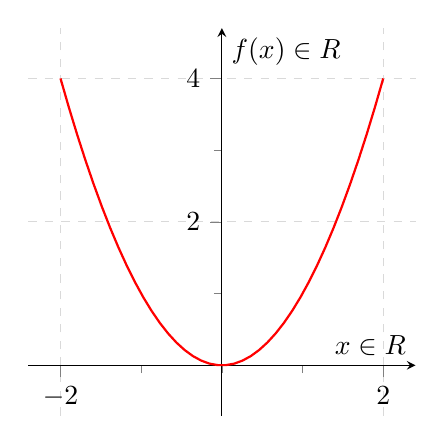
\begin{tikzpicture}
            \begin{axis}[
                legend pos=south west,
                axis x line=middle,
                axis y line=middle,
                grid = major,
                width=6.5cm,
                height=6.5cm,
                grid style={dashed, gray!30},
                xmin=-2,     % start the diagram at this x-coordinate
                xmax= 2,     % end   the diagram at this x-coordinate
                ymin=-0.25,  % start the diagram at this y-coordinate
                ymax= 4.25,  % end   the diagram at this y-coordinate
                axis background/.style={fill=white},
                xlabel=$x \in \mathbb{R}$,
                ylabel=$f(x) \in \mathbb{R}$,
                %xticklabels={-2,-1.6,...,7},
                %yticklabels={-8,-7,...,8},
                tick align=outside,
                minor tick num=-3,
                enlargelimits=true,
                tension=0.08]
              \addplot[domain=-2:2, red, thick,samples=40] {x*x};
            \end{axis}
        \end{tikzpicture}
    }
    \only<2->{
        \pgfplotsset{
            colormap={whitered}{
                color(0cm)=(white);
                color(1cm)=(orange!75!red)
            }
        }
        \begin{tikzpicture}
            \begin{axis}[
            colormap name=whitered,
            width=5.5cm,
            height=5.5cm,
            view={340}{25},
            enlargelimits=false,
            grid=major,
            domain=-3:3,
            y domain=-3:3,
            samples=56, %57 : TeX capacity exceeded, sorry [main memory size=3000000].
                        % see also http://tex.stackexchange.com/a/7954/5645
            xlabel=$x$,
            ylabel=$y$,
            zlabel={$f(x,y)$},
            ]
              \addplot3[surf] {x^2 + y^2};
            \end{axis}
        \end{tikzpicture}
    }
    \end{column}
    \end{columns}
\end{frame}

\begin{frame}{Funktionen mit Parametern}
    \begin{columns}
    \begin{column}{.5\textwidth}
        {\Large Mit Parametern}
        \begin{itemize}[<+->]
            \item $f(x) = x^2$
            \item $f(x) = 2 \cdot x^2$
            \item $f(x) = \nicefrac{1}{2} \cdot x^2$
            \item $f(x) = a \cdot x^2$
            \item $f(x_1, \dots, x_{166}) = \sum_{i=1}^{166} a_i \cdot x_i$\\
                  $\mathbb{R}^{166} \rightarrow \mathbb{R}$
            \item $f(x_1, \dots, x_{166}) = (\sum_{i=1}^{166} a_i \cdot x_i, \dots, \sum_{i=1}^{166} z_i \cdot x_i)$\\
                  $\mathbb{R}^{166} \rightarrow \mathbb{R}^{\text(\# Klassen)}$
        \end{itemize}
    \end{column}
    \begin{column}{.4\textwidth}
        \begin{tikzpicture}
            \begin{axis}[
                legend pos=south west,
                axis x line=middle,
                axis y line=middle,
                grid = major,
                width=6.5cm,
                height=6.5cm,
                grid style={dashed, gray!30},
                xmin=-2,     % start the diagram at this x-coordinate
                xmax= 2,     % end   the diagram at this x-coordinate
                ymin=-0.25,  % start the diagram at this y-coordinate
                ymax= 4.25,  % end   the diagram at this y-coordinate
                axis background/.style={fill=white},
                xlabel=$x \in \mathbb{R}$,
                ylabel=$f(x) \in \mathbb{R}$,
                %xticklabels={-2,-1.6,...,7},
                %yticklabels={-8,-7,...,8},
                tick align=outside,
                minor tick num=-3,
                enlargelimits=true,
                tension=0.08]
              \only<1->{\addplot[domain=-2:2, red, thick,samples=40] {x*x};}
              \only<2->{\addplot[domain=-2:2, blue, thick,samples=40] {2*x*x};}
              \only<3->{\addplot[domain=-2:2, green, thick,samples=40] {0.5*x*x};}
            \end{axis}
        \end{tikzpicture}
    \end{column}
    \end{columns}
\end{frame}

\begin{frame}{Fehlerfunktion}
    \begin{itemize}[<+->]
        \item \textbf{Daten $(x_{i,1}, \dots, x_{i,n}, y_{i,1}, \dots, y_{i,\text{\# Klassen}})$}: Beispiele für den Computer
        \item \textbf{Aktuelles Modell $f$}: Funktion mit vielen Parametern
        \item \textbf{Fehlerfunktion}: Wie gut ist $f$ für die vorhandenen
              Daten?
    \end{itemize}
\end{frame}

\begin{frame}{Fehlerfunktion}
    Abbildung von \textbf{Parameterraum} auf den Fehler ($\mathbb{R}_0^+$)
\end{frame}

\begin{frame}{Minimieren mit Ableitungen}
    \begin{figure}[h]
        \centering
        \includegraphics*[width=0.7\linewidth, keepaspectratio]{images/derivative-function.png}
    \end{figure}
\end{frame}

\begin{frame}{Gradientenabstieg}
    \begin{figure}[h]
        \centering
        \includegraphics*[width=0.7\linewidth, keepaspectratio]{images/gradient-descent.png}
    \end{figure}
\end{frame}


\section{Neuronale Netze}
\subsection{Neuronale Netze}
\begin{frame}{Neuronale Netze}{}
    \begin{itemize}[<+->]
        \item Menge von parametrisierten Funktionen
              $\mathbb{R}^n \rightarrow \mathbb{R}^{\text(\# Klassen)}$
        \item $\mathbb{R}^n$: Eingabe,\\z.B. Farbe von Pixel~1, Farbe von Pixel~2, \dots
        \item $\mathbb{R}^{\text(\# Klassen)}$: Ausgabe,\\Wahrscheinlichkeit der Klasse (z.B. 0, 1, 2, 3, 4, 5, 6, 7, 8, 9)
        \item Ableitbar
    \end{itemize}
\end{frame}

\section{Ausblick}
\subsection{Ausblick}
\begin{frame}{Ausblick}
    Erkennung von Formeln
    \begin{itemize}[<+->]
        \item Aufbau eines Sprachmodells der Mathematik
        \item Erweiterung der Symboldatenbank
        \item Segmentierung
    \end{itemize}
\end{frame}



\section{Preprocessing and Features}
\subsection{Preprocessing}
\begin{frame}{Preprocessing}
    \begin{itemize}
        \item Normalizing
        \begin{itemize}
            \item Scaling
            \item Shifting
            \item Resampling
        \end{itemize}
        \item Noise reduction
        \begin{itemize}
            \item Smoothing (e.g. moving average)
            \item Dot reduction
            \item Filtering (by distance, speed or angle)
            \item Stroke connection
        \end{itemize}
    \end{itemize}
\end{frame}
\subsection{Features}
\begin{frame}{Features}
    \begin{itemize}
        \item Local
        \begin{itemize}
            \item Coordinates
            \item Speed
            \item Binary pen pressure
            \item Direction
            \item Curvature
            \item Bitmap-environment
            \item Hat-Feature
        \end{itemize}
        \item Global
        \begin{itemize}
            \item \# of points
            \item \# of strokes
            \item Center point
            \item Bitmap
            \item Bounding box (width, height, time)
        \end{itemize}
    \end{itemize}
\end{frame}

\section{Evaluation}
\subsection{Evaluation}
\begin{frame}{Baseline Systems}
    \textbf{Preprocessing:} Scaling, shifting and linear interpolation\\
    \textbf{Features:} Coordinates of 80 points (4 strokes with 20 points each)\\
    \textbf{Learning:} MLP, 1000 epochs, LR $\eta=0.1$, Momentum $\alpha=0.1$
\begin{table}[h]
    \centering
    \begin{tabular}{clrrr}
    \toprule
    \multirow{2}{*}{System}  & \multirow{2}{*}{Topology} & \multicolumn{3}{c}{Classification error}\\
          &                         & TOP1                   & TOP3                  & MER \\\midrule
    $B_1$ & 160:500:369             & $\SI{23.34}{\percent}$ & $\SI{6.80}{\percent}$ & $\SI{6.64}{\percent}$ \\
    $B_2$ & 160:500:500:369         & \underline{$\SI{21.51}{\percent}$} & $\SI{5.75}{\percent}$ & $\SI{5.67}{\percent}$ \\
    $B_3$ & 160:500:500:500:369     & $\SI{21.93}{\percent}$ & \underline{$\SI{5.74}{\percent}$} & \underline{$\SI{5.64}{\percent}$} \\
    % $B_4$ & 160:500:500:500:500:369 & $\SI{23.88}{\percent}$ & $\SI{6.12}{\percent}$ & $\SI{6.04}{\percent}$ \\
    \bottomrule
    \end{tabular}
    \caption{Baseline systems with three different classification error measures.
             All errors were measured on the test set.}
\label{table:baseline-systems}
\end{table}
\end{frame}

\subsection{Merged Symbols}
\begin{frame}[fragile]{Merged symbols (MER error)}
\begin{table}[ht]
    \centering
    \begin{tabular}{lc|lc}
        \toprule
        \multicolumn{2}{c}{Base symbol} & \multicolumn{2}{c}{equivalent symbols}\\
        \LaTeX         & Rendered       & \LaTeX                 & Rendered  \\\midrule
        \verb+\sum+    & $\sum$         & \verb+$\Sigma$+        & $\Sigma$\\
        \verb+\prod+   & $\prod$        & \verb+$\Pi$+           & $\Pi$\\
        ~              & ~              & \verb+$\sqcap$+        & $\sqcap$\\
        \verb+\coprod+ & $\coprod$      & \verb+$\amalg$+        & $\amalg$\\
        ~              & ~              & \verb+$\sqcup$+        & $\sqcup$\\
        \verb+\perp+   & $\perp$        & \verb+$\bot$+          & $\bot$\\
        \verb+\models+ & $\models$      & \verb+$\vDash$+        & $\vDash$\\
        \verb+|+       & |              & \verb+\mid+            & $\mid$  \\
        \verb+\Delta+  & $\Delta$       & \verb+$\triangle$+     & $\triangle$\\
        ~              & ~              & \verb+$\vartriangle$+  & $\vartriangle$\\
        \bottomrule
    \end{tabular}
\end{table}
\end{frame}

\begin{frame}[fragile]{Merged symbols (MER error)}
\begin{table}[ht]
    \centering
    \begin{tabular}{lc|lc}
        \toprule
        \multicolumn{2}{c}{Base symbol} & \multicolumn{2}{c}{equivalent symbols}\\
        \LaTeX         & Rendered       & \LaTeX                 & Rendered  \\\midrule
        \verb+\|+      & $\|$           & \verb+$\parallel$+     & $\parallel$\\
        \verb+\ohm+    & $\Omega$         & \verb+$\Omega$+      & $\Omega$\\
        \verb+\setminus+ & $\setminus$  & \verb+$\backslash$+    & $\backslash$\\
        \verb+\checked+ & {\mbox {\wasyfamily \char 8}} & \verb+$\checkmark$+    & $\checkmark$\\
        \verb+\&+      & $\&$           & \verb+$\with$+         & $\&$\\
        \verb+\#+      & $\#$           & \verb+$\sharp$+        & $\sharp$\\
        \verb+\S+      & $\S$           & \verb+$\mathsection$+  & $\mathsection$\\
        \verb+\nabla+  & $\nabla$       & \verb+\triangledown+   & $\triangledown$\\
        \verb+\lhd+    & $\lhd$         & \verb+$\triangleleft$+ & $\triangleleft$\\
        ~              & ~              & \verb+$\vartriangleleft$+ & $\vartriangleleft$\\
        \verb+\oiint+  & $\oiint$       & \verb+$\varoiint$+     & $\varoiint$\\
        \bottomrule
    \end{tabular}
\end{table}
\end{frame}


\begin{frame}[fragile]{Merged symbols (MER error)}
\begin{table}[ht]
    \centering
    \begin{tabular}{lc|lc}
        \toprule
        \multicolumn{2}{c}{Base symbol} & \multicolumn{2}{c}{equivalent symbols}\\
        \LaTeX         & Rendered       & \LaTeX                 & Rendered  \\\midrule
        \verb+\mathbb{R}+ & $\mathbb{R}$ & \verb+$\mathds{R}$+   & $\mathds{R}$\\
        \verb+\mathbb{Q}+ & $\mathbb{Q}$ & \verb+\mathds{Q}+     & $\mathds{Q}$\\
        \verb+\mathbb{Z}+ & $\mathbb{Z}$ & \verb+\mathds{Z}+     & $\mathds{Z}$\\
        \verb+\mathcal{A}+ & $\mathcal{A}$ & \verb+\mathscr{A}+  & $\mathscr{A}$\\
        \verb+\mathcal{D}+ & $\mathcal{D}$ & \verb+\mathscr{D}+  & $\mathscr{D}$\\
        \verb+\mathcal{N}+ & $\mathcal{N}$ & \verb+\mathscr{N}+  & $\mathscr{N}$\\
        \verb+\mathcal{R}+ & $\mathcal{R}$ & \verb+\mathscr{R}+  & $\mathscr{R}$\\
        \verb+\propto+ & $\propto$      & \verb+$\varpropto$+    & $\varpropto$\\
        \bottomrule
    \end{tabular}
\end{table}
\end{frame}

\subsection{Evaluation}
\begin{frame}{Preprocessing: Connect strokes}
\begin{table}[h]
    \centering
    \begin{tabular}{lrrrrrr}
    \toprule
    \multirow{2}{*}{System} & \multicolumn{6}{c}{Classification error}\\
    \cmidrule(l){2-7}
                                         & TOP1                   & change                 & TOP3                   & change                 & MER                & change \\\midrule
    $B_{1,\theta = \SI{5}{\pixel}}$ & $\SI{23.27}{\percent}$ & $\SI{-0.07}{\percent}$ &  $\SI{6.50}{\percent}$ & $\SI{-0.30}{\percent}$ & $\SI{6.37}{\percent}$ & $\SI{-0.27}{\percent}$ \\
    $B_{2,\theta = \SI{5}{\pixel}}$ & $\SI{21.20}{\percent}$ & $\SI{-0.31}{\percent}$ &  $\SI{5.59}{\percent}$ & $\SI{-0.16}{\percent}$ & $\SI{5.50}{\percent}$ & $\SI{-0.17}{\percent}$ \\
    $B_{3,\theta = \SI{5}{\pixel}}$ & $\SI{21.80}{\percent}$ & $\SI{-0.13}{\percent}$ &  $\SI{5.54}{\percent}$ & $\SI{-0.20}{\percent}$ & $\SI{5.47}{\percent}$ & $\SI{-0.17}{\percent}$ \\\midrule
    $B_{1,\theta = \SI{10}{\pixel}}$& $\SI{23.17}{\percent}$ & $\SI{-0.17}{\percent}$ &  $\SI{6.61}{\percent}$ & $\SI{-0.19}{\percent}$ & $\SI{6.47}{\percent}$ & $\SI{-0.17}{\percent}$ \\
    $B_{2,\theta = \SI{10}{\pixel}}$& \underline{$\SI{20.97}{\percent}$} & $\SI{-0.54}{\percent}$ &  $\SI{5.43}{\percent}$ & $\SI{-0.32}{\percent}$ & $\SI{5.34}{\percent}$ & $\SI{-0.33}{\percent}$ \\
    $B_{3,\theta = \SI{10}{\pixel}}$& $\SI{21.34}{\percent}$ & $\SI{-0.59}{\percent}$ & \underline{$\SI{5.42}{\percent}$} & $\SI{-0.32}{\percent}$ & \underline{$\SI{5.33}{\percent}$} & $\SI{-0.31}{\percent}$ \\\midrule
    $B_{1,\theta = \SI{20}{\pixel}}$& $\SI{22.81}{\percent}$ & $\SI{-0.53}{\percent}$ &  $\SI{6.28}{\percent}$ & $\SI{-0.52}{\percent}$ & $\SI{6.19}{\percent}$ & $\SI{-0.45}{\percent}$ \\
    $B_{2,\theta = \SI{20}{\pixel}}$& $\SI{21.61}{\percent}$ & $\SI{+0.10}{\percent}$ &  $\SI{5.79}{\percent}$ & $\SI{+0.04}{\percent}$ & $\SI{5.69}{\percent}$ & $\SI{+0.02}{\percent}$ \\
    $B_{3,\theta = \SI{20}{\pixel}}$& $\SI{21.71}{\percent}$ & $\SI{-0.22}{\percent}$ &  $\SI{5.55}{\percent}$ & $\SI{-0.19}{\percent}$ & $\SI{5.45}{\percent}$ & $\SI{-0.19}{\percent}$ \\
    \bottomrule
    \end{tabular}
    \caption{Models $B_1$--$B_4$ with additionally applied stroke
             connect algorithm.}
\label{table:stroke-connect-evaluation}
\end{table}
\end{frame}

\begin{frame}{Learning: Supervised layer-wise pretraining}
\begin{table}[tb]
    \centering
    \begin{tabular}{lrrrrrr}
    \toprule
    \multirow{2}{*}{System}& \multicolumn{6}{c}{Classification error}\\
    \cmidrule(l){2-7}
              & TOP1                   & change                 & TOP3                  & change                 & MER                & change \\\midrule
    $B_1$     & $\SI{23.34}{\percent}$ &                        & $\SI{6.80}{\percent}$ &                        & $\SI{6.64}{\percent}$ & \\%chktex 8
    $B_{2,p}$ & $\SI{19.89}{\percent}$ & $\SI{-1.62}{\percent}$ & $\SI{4.76}{\percent}$ & $\SI{-0.99}{\percent}$ & $\SI{4.68}{\percent}$ & $\SI{-0.99}{\percent}$\\
    $B_{3,p}$ & \underline{$\SI{19.43}{\percent}$} & $\SI{-2.50}{\percent}$ & \underline{$\SI{4.64}{\percent}$} & $\SI{-1.10}{\percent}$ & \underline{$\SI{4.54}{\percent}$} & $\SI{-1.10}{\percent}$\\
    % $B_{4,p}$ (pretrained) & $\SI{19.63}{\percent}$ & $\SI{-4.25}{\percent}$ & $\SI{4.66}{\percent}$ & $\SI{-1.46}{\percent}$ & $\SI{4.55}{\percent}$ & $\SI{-1.49}{\percent}$\\
    \bottomrule
    \end{tabular}
    \caption{Supervised layer-wise pretraining, 1000 epochs per layer}
\label{table:pretraining-copy-before}
\end{table}
\end{frame}

\definecolor{light-gray}{gray}{0.70}

\subsection{Optimized classifier}
\begin{frame}{Optimized classifier}
    \textbf{Preprocessing:} Connect strokes{\color{light-gray}, scale, shift and linear interpolation}\\
    \textbf{Features:} {\color{light-gray}Coordinates of 80 points (4 strokes with 20 points each),} re-curvature per stroke, ink, stroke count, aspect ratio\\
    \textbf{Learning:} {\color{light-gray}MLP, 1000 epochs, LR $\eta=0.1$, Momentum $\alpha=0.1$,} supervised layer-wise pretraining
\begin{table}[htb]
    \centering
    \begin{tabular}{lrrrrrr}
    \toprule
    \multirow{2}{*}{System}  & \multicolumn{6}{c}{Classification error}\\
    \cmidrule(l){2-7}
              & TOP1                   & change                 & TOP3                  & change                 & MER                   & change \\\midrule
    $B_{1,c}$ & $\SI{20.96}{\percent}$ & $\SI{-2.38}{\percent}$ & $\SI{5.24}{\percent}$ & $\SI{-1.56}{\percent}$ & $\SI{5.13}{\percent}$ & $\SI{-1.51}{\percent}$ \\
    $B_{2,c}$ & $\SI{18.26}{\percent}$ & $\SI{-3.25}{\percent}$ & $\SI{4.07}{\percent}$ & $\SI{-1.68}{\percent}$ & \underline{$\SI{3.98}{\percent}$} & $\SI{-1.69}{\percent}$ \\
    $B_{3,c}$ & \underline{$\SI{18.19}{\percent}$} & $\SI{-3.74}{\percent}$ & \underline{$\SI{4.06}{\percent}$} & $\SI{-1.68}{\percent}$ & $\SI{3.99}{\percent}$ & $\SI{-1.65}{\percent}$ \\
    % $B_{4,c}$ & $\SI{18.57}{\percent}$ & $\SI{-5.31}{\percent}$ & $\SI{4.25}{\percent}$ & $\SI{-1.87}{\percent}$ & $\SI{4.18}{\percent}$ & $\SI{-1.86}{\percent}$ \\
    \bottomrule
    \end{tabular}
    \caption{Error rates of the complex recognizer systems.}
\label{table:complex-recognizer-systems-evaluation}
\end{table}
\end{frame}

\section*{End}
\subsection{End}
\subsection{Sources}
\begin{frame}{Folien}
    Die Folien sind unter \url{tinyurl.com/gute-frage-sq} (\url{https://github.com/MartinThoma/LaTeX-examples/tree/master/presentations/Gute-Frage-Schluesselqualifikation})
    verfügbar.
\end{frame}
\framedgraphic{Thanks for Your Attention!}{../images/xi.png}

\end{document}
